\subsection*{Иродов 2.244}
\setcounter{equation}{0}

\begin{abstract}
Ток $I$ течет по длинному проводу и затем растекается равномерно по всем направлениям в однородной проводящей среде (рис. 2.73). Пренебрегая влиянием вещества среды, найти индукцию магнитного поля в точке A, отстоящей от точки O на расстояние $r$ под углом $\theta$.
\end{abstract}

\noindent \hrulefill
\\
\begin{wrapfigure}[6]{r}{0.30\textwidth}
	\raisebox{0pt}[\dimexpr\height-2\baselineskip\relax]{
	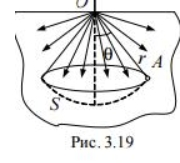
\includegraphics[width=0.30\textwidth]{pics/2_244.jpeg}}
\end{wrapfigure}

Рассмотрим окружность, расположенную в сфере под углом $\theta$, радиус которой равен $r \sin{\theta}$. Благодаря симметрии магнитная индукция $B$ постоянна и направлена по касательной к окружности.

Согласно теореме Ампера:

$$\oint_C \vec{B} \, \vec{(d \ell)} = \mu_0 I'$$

($I'$ - ток , который проходит через область, ограниченную этой окружности)

$$\xrightarrow{} B.2 \pi r \sin{\theta} = \mu_0 I' \quad (1)$$

Ток от O равномерно распространяется в пространстве, поэтому:

$$I' = I .\frac{S}{2 \pi r^2} \quad (2)$$

($S$ - площадь поверхности конуса, которая содержит угол $\theta$)

$$S = r^2. \Omega = r^2  \int_0^{2 \pi} d \phi  \int_0^{\theta} \sin{\theta'}\, d\theta' = r^2 2 \pi (1-\cos{\theta})$$

$$\xrightarrow{(2)} I' = I (1- \cos{\theta})$$

$$\xrightarrow{(1)} B(r) = \frac{\mu_0}{2 \pi r \sin{\theta}} I (1 - \cos{\theta}) = \frac{\mu_0 I}{2 \pi r}  \tan{\frac{\theta}{2}}$$

\textbf{Ответ:}

$$ B(r) =  \frac{\mu_0 I}{2 \pi r}  \tan{\frac{\theta}{2}}$$









